%================================================================
%                           N O T E S
%                           ---------
%
%                           ---------
%-----------------------------------------------------------------
%                       INTRODUCTION
%-----------------------------------------------------------------
\section{Introduction to the problem}
For this problem we consider a plane wave propagates from infinity onto a cylinder centered at the origin and of radius $\sigma$, as depicted in \figref{fig:problem_1}. We will attempt to find an expression for the velocity field of this wave as it scatters around the cylinder. We will consider two different boundary conditions, Neumann and Dirichlet, and will find expressions for both of these. \par
%
    \begin{figure}
        \centering
        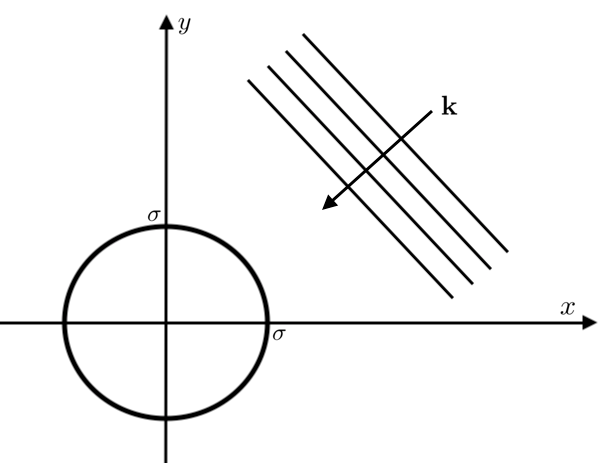
\includegraphics[width=6cm]{../figures/sk_problem_1.png}
        \caption{Problem 1}
        \label{fig:problem_1}
    \end{figure}
%
Throughout this problem we will be concerned with finding an expression for the total velocity field around the cylinder, $\vec{u}$. As we showed in \ssref{ss:physical_interpretation}, it will be sufficient for us to seek $\Phi(x, y)$, since this is a 2D problem. \par
%
Let $\Phitot = \Phiin + \Phisc$, where $\Phiin$ is the incident field, and $\Phisc$ is the scattered field. All three of these must satisfy the Helmholtz equation.
%====================================================================
%                   INCIDENT FIELD
%====================================================================
\section{The incident field}
First let us consider $\Phiin$, the incident field. We choose Cartesian coordinates $(x,y)$, and polar coordinates $(r, \theta)$.
    \begin{propn}\label{propn:ch2_inc_field_intro}
    The incident field has the form
        \begin{equation}
            \Phiin = e^{-i(\vec{k}\cdot\vec{x})}
        \end{equation}
    \end{propn}
    \begin{proof}
    We need to show that this expression for $\Phiin$ satisfies the Helmholtz equation, \eqref{eq:helmholtz}. \par
        \begin{align*}
            \nabla^2 \Phiin
            &= \left[ \partialfrac{^2}{x^2} + \partialfrac{^2}{y^2} \right] e^{-i(\vec{k}\cdot\vec{x})} \\
            &= (-i)^2 a^2 e^{-i(ax+by)} + (-i)^2b^2 e^{-i(ax+by)}\\
            &= -(a^2+b^2)\Phiin
        \end{align*}
    Then,
        \begin{gather*}
            \nabla^2 \Phiin + k^2 \Phiin
            = -(a^2+b^2)\Phiin + k^2 \Phiin = 0\\
            \Rightarrow k^2-(a^2+b^2)=0
        \end{gather*}
    which is true by definition of the wave vector $\vec{k}$ (see definition \ref{defn:wave_vector}).
    \end{proof}

%
    \begin{propn}\label{propn:ch2_inc_field_infty_sum}
    The incident field can be expressed as an infinite sum as follows.
        \begin{equation*}\label{eq:ch2_inc_field_infty_sum}
            \Phiin = \sum^{\infty}_{n=0} \epsilon_n i^n J_n(kr) \cos (n(\theta - \alpha))
        \end{equation*}
    \end{propn}
    \begin{proof}
    Follows directly from Propositions \ref{propn:ch2_inc_field_intro} and  \ref{propn:jacobi_expansion}.
    \end{proof}
%-----------------------------------------------------------------
%                       SCATTERED FIELD
%-----------------------------------------------------------------
\section{The scattered field}\label{ss:scattered_field}
To find the expression for the scattered field we will again use the method of separation of variables. We make two assumptions for the potential $\Phisc$:
\begin{enumerate}[label=(\roman*)]
  \item it is separable into two indepdent functions, one for $r$ and one for $\theta$, and
  \item it satisfies the Helmholtz equation.
\end{enumerate}
%
\begin{propn}\label{propn:scattered_field_differential_equations}
  With these two assumptions, we get two independent differential equations to solve to find the radial and azimuthal components of the velocity field.
  %
  \begin{equation}\label{eq:ch2_theta_dep}
      \frac{d^2 \Theta}{d\theta^2} + \hat{\nu} \Theta = 0, ~\text{and}
  \end{equation}
  %
  \begin{equation}\label{eq:ch2_r_dep}
      r^2 \frac{d^2 R}{dr^2} + r \frac{d R}{dr} + (k^2r^2 - \hat{\nu}) R = 0.
  \end{equation}
  %
  Where $\hat{\nu} \in \bb{C}$.
\end{propn}
%
\begin{proof}
  From assumption (i) we have
  \begin{equation}
      \Phisc = R(r) \Theta(\theta),
  \end{equation}\par
  %
  and from (ii)
  \begin{equation}\label{eq:phisc_helmholtz}
      \nabla^2 \Phisc + k^2 \Phisc = 0.
  \end{equation}
  %
  Hence,
  \begin{align*}
      \frac{1}{r} \partialfrac{}{r}
      \left( r \partialfrac{}{r} [R(r) \Theta(\theta)] \right)
      &+ \frac{1}{r^2} \partialfrac{^2}{\theta^2} [R(r) \Theta(\theta)]
      + k^2 R(r) \Theta(\theta) = 0 \\
      %
      \Theta(\theta) \left( \frac{1}{r} \frac{dR(r)}{dr} + \frac{d^2 R(r)}{dr^2} \right)
      &+ \frac{R(r)}{r^2} \left( \frac{d^2 \Theta(\theta)}{d\theta^2}\right)
      + k^2 R(r) \Theta(\theta) = 0 \\
      %
      \Theta \left( \frac{1}{r} R' + R''\right)
      &+ \frac{1}{r^2} R \Theta'' + k^2 R \Theta = 0
  \end{align*}
  \begin{equation*}
       r^2 \frac{R''}{R} + r\frac{R'}{R} + (kr)^2 = - \frac{\Theta''}{\Theta}
  \end{equation*}\par
  %
  For this to be true we must have the left hand side and the right hand side equal to the same constant, $\hat{\nu}$. That is,
  \begin{gather*}
    r^2 \frac{R''}{R} + r\frac{R'}{R} + (kr)^2 = \hat{\nu} \\
    %
    \text{and } \frac{\Theta''}{\Theta} = - \hat{\nu}
  \end{gather*}
  as required.
\end{proof}

%-------------------- principle of superposition ---------------------

\begin{thm}The principle of superposition for second order homogeneous linear equations is that statement that if $y_1$ and $y_2$ are any two solutions to the equation
  \[ \ddot{y} + p(t)\dot{y} + q(t)y =  0\]
  then any function of the form
  $ y_0 = C_1 y_1 + C_2 y_2 $
  is also a solution of the equation.
\end{thm}
\begin{proof}
  Consider the function $y_0$ as defined above. Then
  \begin{gather*}
    \dot{y}_0 = C_1 \dot{y}_1 + C_2 \dot{y}_2 \\
    \ddot{y}_0 = C_1 \ddot{y}_1 + C_2 \ddot{y}_2.
  \end{gather*}
  So the ODE becomes
  \begin{gather*}
    C_1 \ddot{y}_1 + C_2 \ddot{y}_2 + p(t) [ C_1 \dot{y}_1 + C_2 \dot{y}_2 ] + q(t) [C_1 y_1 + C_2 y_2] = 0
  \end{gather*}
  which holds if and only if
  \begin{gather*}
    \left\{
    \begin{array}{l}
      C_1[\ddot{y_1} + p(t)\dot{y_1} + q(t)y_1] =  0 ~~\text{and}\\
      C_2[\ddot{y_2} + p(t)\dot{y_2} + q(t)y_2] =  0.
    \end{array}
    \right.
  \end{gather*}
  By definition, $y_1$ and $y_2$ are solutions to the ODE, therefore $ y_0 = C_1 y_1 + C_2 y_2 $ is also a solution for any constants $C_1$, $C_2$ as required.
\end{proof}
%=====================================================================
%           propn: general solution for angular dependence
%=====================================================================
\begin{propn}
  The expression
  \[
  \Theta(\theta) = \sum_{n=0}^{\infty} A_n \cos(n\theta) + B_n \sin(n\theta)
  \]
  is a general solution to \eqref{eq:ch2_theta_dep}.
\end{propn}
\begin{proof}
  Firstly, we want to show that $\nu = n \in \bb{Z}.$ We consider three cases. \par
  %
  \textbf{Case 1.} Let $\hat{\nu} = 0$. This gives a linear solution:
      \begin{equation}
          \Theta(\theta) = A_1 \theta + B_1.
      \end{equation}\par
  %
  \textbf{Case 2.} Let $\hat{\nu} = \nu^2 < 0.$ Then we get an solution of exponential form.:
      \begin{equation}
          \Theta(\theta) = A_2 e^{\nu \theta} + B_2 e^{- \nu \theta}.
      \end{equation}\par
  %
  \textbf{Case 3.} Let $\hat{\nu}= - \nu^2 < 0$. This gives a solution of trigonometric form:
      \begin{equation}
          \Theta(\theta) = A_3 \cos(\nu\theta) + B_3 \sin(\nu\theta).
      \end{equation}\par
  %
  Since $\theta$ is the polar angular coordinate, we expect our solution to be $2\pi$ periodic. We can therefore discount Case 2. Case 1 is only periodic in the trivial case where $A_1 = 0$, and this is included in Case 3. We can therefore assume that $\hat{\nu} = - \nu^2 \leq 0$. \par
  %
  Since our solution must be $2\pi$ periodic, we have
  \begin{align*}
    \Theta(\theta) &= \Theta(\theta+2 \pi)\\
    A \cos(\nu\theta) + B \sin(\nu \theta) &= A \cos(\nu\theta+2\pi\nu) + B \sin(\nu \theta + 2 \pi \nu)
  \end{align*}
  %
  \begin{multline*}
      A \cos(\nu\theta) + B \sin(\nu \theta) \\
      = A [\cos(\nu\theta)\cos(2\pi\nu) - \sin(2\pi\nu)\sin(\nu\theta)] \\
      + B [\sin(\nu\theta)\cos(2\pi\nu) + \cos(\nu\theta)\sin(2\pi\nu)]
  \end{multline*}
  %
  \begin{multline*}
      \therefore A\cos(\nu\theta) + B \sin(\nu \theta) \\
      = \cos(\nu\theta)[A\cos(2\pi\nu) + B\sin(2\pi\nu)] \\
      + \sin(\nu\theta)[B\cos(2\pi\nu) - A\sin(2\pi\nu)]
  \end{multline*}\par
  %
  So we have
  \begin{align*}
    A &= A\cos(2\pi\nu) + B\sin(2\pi\nu) \text{ and}\\
    B &= B\cos(2\pi\nu) - A\sin(2\pi\nu).
  \end{align*}\par
  %
  Or equivalently,
  \begin{align}\label{eq:eigenvalue_proof_angular_dep}
    \begin{pmatrix}
      1 - \cos(2\pi\nu) & -\sin(2\pi\nu)\\
      \sin(2\pi\nu) & 1 - \cos(2\pi\nu)
    \end{pmatrix}
    \begin{pmatrix}
      A\\
      B
    \end{pmatrix}
    = 0
  \end{align}\par
  %
  We'll call the matrix on the left hand side $\mathbf{M}$. For \eqref{eq:eigenvalue_proof_angular_dep} to be true, $\det(\mathbf{M}) = 0$, and so
  \begin{gather*}
    (1 - \cos(2\pi\nu))^2 + (\sin(2\pi\nu))^2 = 0 \\
    1 - 2\cos(2\pi\nu) + \cos^2(2\pi\nu) + \sin^2(2\pi\nu) = 0 \\
    2 - 2\cos(2\pi\nu) = 0 \\
    \cos(2\pi\nu) = 1
  \end{gather*}\par
  %
  Hence $\nu = n \in \bb{Z}$ as required. \par
  %
  We have therefore shown that
  \begin{equation}
    A \cos(n\theta) + B \sin(n \theta)
  \end{equation}
  are particular solutions to \eqref{eq:ch2_theta_dep} for all $A, B$ constants and $n \in \bb{Z}.$ Hence by the principle of superposition, any linear combination of these is also a soltion to \eqref{eq:ch2_theta_dep}. Hence we have the general solution
  \begin{equation*}
    \sum_{n=0}^\infty A_n \cos(n\theta) + B_n \sin(n \theta)
  \end{equation*}
  for $A_n, B_n$ constants as required.
\end{proof}

We now seek a solution to the radial component of this field. We now know that $\hat{\nu} = \nu^2$, so we can rewrite \eqref{eq:ch2_r_dep} as follows:
    \begin{equation}\label{eq:ch2_r_dep_2}
        r^2 \frac{d^2 R}{dr^2} + r \frac{d R}{dr} + (k^2r^2 - \nu^2) R = 0.
    \end{equation}
    \begin{propn}
    Equation \eqref{eq:ch2_r_dep_2} is a Bessel differential equation of order $\nu$.
    \end{propn}
    \begin{proof} Consider the substitution $r=kz$. Then
        \begin{align*}
            \frac{dR}{dr} = \frac{1}{k} \frac{dR}{dz}, ~~
            \frac{d^2R}{dr^2} = \frac{1}{k^2} \frac{d^2R}{dz^2}.
        \end{align*}\par
    %
    So \eqref{eq:ch2_r_dep_2} becomes
        \begin{align}
            \frac{r^2}{k^2}\frac{d^2R}{dz^2}
                + \frac{r}{k}\frac{dR}{dz}
                &+ (k^2r^2 - \nu^2)R = 0, \\
            z^2 \frac{d^2 R}{dz^2}
                + z \frac{dR}{dz}
                &+ (z^2 - \nu^2)R = 0.
        \end{align}
    This fits the defintion of the Bessel differential equation \eqref{eq:bessel_differential}.
    \end{proof}

Since $R(kr)$ satisfies a Bessel differential equation, the Bessel functions are solutions, and by the superposition principle any linear superposition of these is also a solution. We will need to consider the Sommerfeld radiation condition in order specify the general solution for $R(r)$.

\begin{defn}\emph{The Sommerfeld radiation condition.} \parencite{martin06scattering} \label{defn:sommerfeld_radiation_condition}
  \[ r^{1/2} \left( \partialfrac{\Phisc}{r} - ik\Phisc \right) \rightarrow 0 \text{ as } r \rightarrow \infty\]
\end{defn}
Naively, the Sommerfeld radiation condition states that wave diffuses as $r\rightarrow\infty$, and that the scattered waves are not reflecting back and incoming from infinity -- something we wouldn't expect to happen physically. It is therefore reasonable to apply this condition to our problem.

From now on we refer to $H^{(1)}_n$ as $H_n$ for simplicity.

\begin{propn}
  Hankel functions of the first kind satisfy the Sommerfeld radiation condition.
\end{propn}
\begin{proof}
  It is known that \parencite{martin06scattering}
  \begin{equation}
    H_n(kr) \sim \sqrt{\frac{2}{\pi kr}} e^{i(kr - \frac{n\pi}{2} - \frac{\pi}{4}}) \text{ as } r \rightarrow \infty
  \end{equation}

  Then as $r\rightarrow\infty$
  \begin{align*}
    &\partialfrac{H_n(kr)}{r}
    \sim \frac{d}{dr} \left\{
    \sqrt{\frac{2}{k\pi}} r^{-1/2} e^{i(kr - n\pi/2- \pi/4)}
    \right\}\\
    &\sim\left\{
    \sqrt{\frac{2}{k\pi}} \frac{d}{dr} (r^{-1/2}) e^{i(kr - n\pi/2- \pi/4)}
    + \sqrt{\frac{2}{k\pi}} r^{-1/2} \frac{d}{dr}(e^{i(kr - n\pi/2- \pi/4)})
    \right\} \\
    &\sim \sqrt{\frac{2}{k\pi}} \left\{
    \left(-\frac{1}{2} \right) r^{-3/2} e^{i(kr - n\pi/2- \pi/4)} + r^{-1/2} (ik) e^{i(kr - n\pi/2- \pi/4)}
    \right\} \\
    &\sim \sqrt{\frac{2}{kr\pi}} e^{i(kr - n\pi/2- \pi/4)} \left\{
    \left(-\frac{1}{2r} \right) + ik
    \right\} \\
    &\sim H_n(kr) \left\{
    \left(-\frac{1}{2r} \right) + ik
    \right\}.
  \end{align*}

  Hence we have
  \begin{align*}
    r^{1/2} \left(
      \partialfrac{H_n(kr)}{r} - ik H_n(kr)
    \right) &\sim r^{1/2} \left(
    H_n(kr) \left\{
    \left(-\frac{1}{2r} \right) + ik - ik
    \right\}
    \right)\\
    & \sim \left(-\frac{1}{2r} \right)
      \sqrt{\frac{2}{k\pi}} e^{i(kr - n\pi/2- \pi/4)} \\
    & \sim -\sqrt{\frac{1}{2kr^2\pi}} e^{i(kr - n\pi/2- \pi/4)}\\
  \end{align*}

  We can now show that this tends to $0$ as $r\rightarrow\infty$, satisfying the Sommerfeld radiation condition. Consider the behaviour real part as $r\rightarrow\infty$
  \begin{align*}
    & \sim -\frac{1}{r} \cos{kr},
  \end{align*}
  and the imaginary part
  \begin{align*}
    & \sim -\frac{1}{r} \sin{kr}.
  \end{align*}

  Both of these tend to $0$ as $r\rightarrow\infty$. Hence we have shown that if $R(r)=H_n(kr)$, $\Phisc$ will satisfy the Sommerfeld radiation condition.
\end{proof}

%----------------------------------------------------------------
%               General solution
%----------------------------------------------------------------
We can now combine our solutions for $\Theta$ and $R$ to find an expression for $\Phisc$.

\begin{propn}\label{eq:gen_sol_scatterin_outside_cylinder}
  The general solution for scattered field can be expressed as follows.
    \begin{equation} \label{eq:ch2_gen_eq_scattered_field}
        \Phisc = \sum^\infty_{n=-\infty} \epsilon_n i^n B_n H_n(kr) \cos(n(\theta-\alpha))
    \end{equation}
  for $B_n$ a constant.
\end{propn}
\begin{proof}
  We have already showed that the radial component of the scalar potential must be a Hankel function. We have also showed that the radial component must be of the form
    \begin{align*}
      A \cos(n\theta) + B \sin(n \theta).
    \end{align*}

  We expect our solution to have the same angular dependence as the incident field, since it is generated by it, so we can set the constants $A,B$ to the following
    \begin{gather*}
      \cos(n\alpha) \cos(n\theta) + \sin(n \alpha) \sin(n \theta)
      = \cos(n(\theta-\alpha)).
    \end{gather*}

  So we have a solution of the form
    \begin{equation}
      C_n H_n(kr) \cos(n(\theta-\alpha)).
    \end{equation}
  for any constant $C_n$. It will be useful when setting the boundary conditions find $ B_n = C_n/\epsilon_n i^n$ instead of $C_n$. So the general solution is
  \begin{equation}
    \sum^\infty_{n=0} \epsilon_n i^n B_n H_n(kr) \cos(n(\theta-\alpha))
  \end{equation}
  as expected.
\end{proof}

%----------------------------------------------------------------
%           ~ B O U N D A R Y  C O N D I T I O N S ~
%----------------------------------------------------------------

\section{Boundary contions}

At the beginning of the chapter we defined
  \[ \Phitot = \Phisc + \Phiin \]
so we can express $\Phitot$ as follows, using \eqref{propn:ch2_inc_field_infty_sum}
\begin{equation}
  \sum^\infty_{n=0} \epsilon_n i^n B_n [H_n(kr) + J_n(kr)] \cos(n(\theta-\alpha)).
\end{equation}

The only thing left to do now is to find the value of $B_n$.

\subsection*{Neumann boundary condition}

We first cosider the boundary at the cylinder wall to satisfy a Neumann boundary condition.
  \begin{defn}
    \parencite[$\S$1.3.2]{martin06scattering} A boundary is sound-hard if
      \begin{align*}
        \partialfrac{u}{r} = 0 \text{,  on } r = \sigma.
      \end{align*}
  \end{defn} \par
%
Equivalently, we can express this boundary condition in terms of $\Phi$:
  \begin{align*}
    \partialfrac{\Phi}{r}=0 \text{,  on } r = \sigma.
  \end{align*} \par
%
We can now apply this to find an expression for the constant terms in \eqref{eq:ch2_gen_eq_scattered_field}. Differentiating this equation gives
  \begin{equation}
    \sum^\infty_{n=0} \epsilon_n k i^n
    \{ J'_n(kr) + B_n H'_n(kr) \} \cos(n(\theta-\alpha)) = 0
  \end{equation}
Since $\cos(n(\theta - \alpha)) \neq 0 ~ \forall n, \theta$, it must be that the expression inside the braces must be zero for each $n$ at the boundary $r=\sigma$. Hence, we get an expression for $B_n$:
  \begin{equation}
    B_n= \frac{J'_n(k\sigma)}{H'_n(k\sigma)}.
  \end{equation}

\subsection*{Dirichlet boundary condition}\label{ss:ch2_dirichlet_bcs}
We now consider the Dirichlet boundary condition.
  \begin{defn}
    \parencite[$\S$1.3.2]{martin06scattering} A body is sound-soft if
      \[
      u = 0 \text{,  on } r = \sigma
      \]
  \end{defn}
Hence, $\Phi_{sc} = - \Phi_{in}$ on $r=\sigma$,
  \begin{align*}
    \sum^\infty_{n=0} \epsilon_n i^n B_n H_n(kr) \cos(n((\theta-\alpha)))
    & = - \sum^\infty_{n=0} \epsilon_n i^n J_n(kr) \cos(n((\theta-\alpha))) \\
    \text{hence for all } n,~ B_n H_n (k\sigma) &= - J_n (k\sigma) \\
  \end{align*}
Hence the Dirichlet boundary condition specifies $B_n$ as follows.
  \begin{equation}
    B_n = \frac{- J_n(k\sigma)}{H_n(k\sigma)}
  \end{equation}

\section{Plotting the solution}
